\documentclass[11pt]{article}
\usepackage[utf8]{inputenc}\usepackage[T1]{fontenc}
\usepackage{amsmath,amssymb,amsthm}\usepackage[margin=1in]{geometry}
\usepackage{graphicx}\usepackage{booktabs}\usepackage{multirow}\usepackage{enumitem}
\usepackage[hidelinks]{hyperref}
\newtheorem{proposition}{Proposition}
\theoremstyle{remark}\newtheorem{remark}{Remark}

\title{Prime Gaps on the $6N$ Skeleton:\\
An $\omega$-Dependent Shift in the Twin-Prime Gap Distribution,\\
and a Congruence-Lockdown Mechanism}
\author{Ruqing Chen\\
\small GUT Geoservice Inc., Montreal, Quebec, Canada\\
\small \texttt{ruqing@hotmail.com}}
\date{\today}

\begin{document}
\maketitle

\begin{abstract}
In Part~I we showed that the conditional density of twin primes on the
$6N\pm1$ skeleton depends on the factorisation of the centre $N$ through the
local enrichment factor $E(N)=\prod_{q\mid N,\,q>3}(q-1)/(q-3)$. Here we ask the
complementary question: not how many twin centres survive, but how they are
\emph{spaced}. Using the exact set of $23{,}988{,}173$ twin centres in the decade
shell $S_{10}$ (where $6N\in[10^{9},10^{10})$) (and the corresponding sets in
$S_8,S_9$), we study the
distribution of the gap $\Delta N$ between consecutive twin centres, stratified
by $\omega_{>3}(N)$, the number of distinct prime factors $>3$ of the left
centre. The aggregate gap distribution is the known Hardy--Littlewood shape,
peaking at the highly divisible values $6\Delta N=30,42,210$. The new finding is
that the \emph{shape} shifts systematically with $\omega_{>3}$: the relative
preference for the short gap $6\Delta N=42$ rises monotonically with $\omega$
(from $0.73$ to $1.55$ across $\omega=1$--$6$ in $S_{10}$) while that for
$6\Delta N=210$ falls (from $1.15$ to $0.41$); the trend reproduces across
$S_8,S_9,S_{10}$ over a $\sim\!64\times$ range of sample size. This contradicts
the \emph{unconditional} Hardy--Littlewood prediction, in which gap preference
depends only on the gap and not on the centre. We identify a first-order
mechanism---\emph{congruence lockdown}: each prime factor $q$ of the centre
forbids the gap residues $\Delta N\equiv\pm6^{-1}\pmod q$---which quantitatively
reproduces the rise of $42$ and $30$ and the collapse of the absolute survival
of $210$, but leaves a genuine residual at high $\omega$. We make no claim about
the infinitude of twin primes. The closed-form conditional gap singular series,
and the high-$\omega$ residual, are posed as open problems.
\end{abstract}

\noindent\textbf{Keywords:} twin primes, prime gaps, Hardy--Littlewood singular
series, jumping champions, conditional density, $6N\pm1$ framework.

\section{Introduction}

The coarse statistics of prime gaps are classically governed by gap-only laws.
The most common gap between consecutive primes up to $x$---the \emph{jumping
champion}---was conjectured by Odlyzko, Rubinstein and Wolf~\cite{ORW} to be $4$
and the primorials $2,6,30,210,2310,\dots$, with $6$ reigning until
$x\approx1.74\times10^{35}$, where $30$ takes over, and $210$ only far beyond.
Goldston and Ledoan~\cite{GL} proved, on the Hardy--Littlewood prime $k$-tuple
conjecture, that sufficiently large jumping champions are primorials. The
mechanism in all this work is the singular series for a gap $d$,
\[
  \mathfrak{S}(d)=2C_2\prod_{\substack{p\mid d\\ p>2}}\frac{p-1}{p-2},
  \qquad C_2=0.6601\ldots,
\]
which grows fastest along the primorials and so makes highly divisible gaps the
most common. The decisive structural feature is that $\mathfrak{S}(d)$ depends
\emph{only on the gap $d$}: it is blind to where on the number line the gap sits,
and in particular to the arithmetic of the integers bracketing it.

In Part~I~\cite{ChenI} we studied a different, conditional, layer of structure.
Restricting to the $6N\pm1$ skeleton and stratifying centres $N$ by their
arithmetic ``pressure'' $\omega_{>3}(N)$ (the number of distinct prime factors
$q>3$ of $N$), we derived and validated the local enrichment factor
$E(N)=\prod_{q\mid N,\,q>3}(q-1)/(q-3)$ governing the conditional probability
that $6N\pm1$ are both prime, and showed it reproduces the squarefree bias of
Puszkarz~\cite{Pusz}. That work answered ``how many'' twin centres occur at a
given factor structure.

The interplay between prime factorisation and gaps has been approached before,
along three avenues that we are careful to distinguish from ours. \emph{(a)
Empirical twin-gap models.} Kelly and Pilling~\cite{KP1,KP2} built, from twin
primes below $2\times10^{11}$, an empirical model of the gap distribution,
finding a single unconditional exponential law $\mathcal P(s)=m\,e^{-ms}$ whose
decay parameter $m$ depends only on the scale $N$, and analysing the ``high
jumper'' (most probable separation). Crucially, their separation $s$ is counted
\emph{within the sequence of primes} (singletons between twins) and their model
carries no dependence on the factorisation of any centre. \emph{(b) Gaps between
almost-primes.} Goldston, Graham, Pintz and Yıldırım~\cite{GGPY}, and
subsequently Sono~\cite{Sono}, used sieve methods to bound small gaps between
$E_2$-numbers (integers with exactly two prime factors); there the factor count
constrains the \emph{endpoints} of the gap, and the endpoints are almost-primes,
not twin primes. \emph{(c) Harmonic/sieve density estimates.}
Dolgikh~\cite{Dolgikh} used prime ``harmonics'' (modulo cycles) to obtain
heuristic lower bounds on the absolute density of twin pairs, in service of
existence questions. Our study departs from all three: we do not model the
unconditional distribution, nor constrain endpoints, nor estimate global
density. We perform a conditional, empirical tomography of the gaps between
\emph{true} twin pairs, stratifying by the factor count $\omega_{>3}(N)$ of the
skeleton \emph{centre} $N$, and we ask how the gap-distribution \emph{shape}
varies across these strata. To our knowledge this conditioning variable---the
arithmetic of the centre rather than of the endpoints or the global scale---has
not previously been used to resolve the twin-gap distribution.

This paper answers ``how far apart''. For consecutive twin centres
$N_i<N_{i+1}$ we study the gap $\Delta N=N_{i+1}-N_i$ (in centre-step units; the
physical distance between the pairs is $6\Delta N$). The question is whether the
gap distribution, like the jumping-champion law, depends only on $\Delta N$, or
whether---as Part~I might suggest---it also depends on the factor structure of
the centres. We find the latter, and we trace it to a concrete conditional
mechanism. Three deliberately bounded claims are made:
\begin{enumerate}[label=(\roman*)]
  \item the twin-gap distribution exhibits a monotone, scale-stable dependence
        on $\omega_{>3}(N)$ (\S2), which the unconditional Hardy--Littlewood
        series cannot produce;
  \item a first-order \emph{congruence-lockdown} mechanism quantitatively
        explains most of it---the rise of the short gaps $42,30$ and the
        collapse of the long gap $210$ (\S3);
  \item a residual at high $\omega$ remains, which we pose, with the closed-form
        conditional singular series, as an open problem (\S3).
\end{enumerate}
Nothing here bears on the infinitude of twin primes. As in Part~I, the headline
phenomenon sits on prior work (the primorial gap preference is the
jumping-champion effect of \cite{ORW}); our contribution is the conditional,
$\omega$-resolved layer and its mechanism.

\paragraph{Data.}
All statistics come from an exhaustive scan of the $6N\pm1$ skeleton with
complete factorisation and deterministic interval-sieve primality; the $S_{10}$
twin count $23{,}988{,}173$ matches Part~I to the integer. Gaps spanning a shell
boundary are discarded so that $\log(6N)$ is effectively constant within each
stratum. Code and data are released openly~\cite{repo2}.

\section{The $\omega$-dependence of the gap distribution}

\subsection{The aggregate distribution is the known shape}
Aggregated over all centres, the gap distribution in $S_{10}$ peaks exactly where
the jumping-champion law predicts: the most frequent gaps are $6\Delta N=30$
($2.45\%$), $42$ ($2.28\%$), then $90,60,210,\dots$---the highly divisible
values. We confirmed (Part~II companion computation) that this aggregate shape is
reproduced to correlation $0.999$ by the two-endpoint Hardy--Littlewood
correlation factor $C_2(\Delta N)$ times an $\omega$-independent geometric
envelope. At the aggregate level there is nothing new: the primorial preference
is the known effect.

\subsection{The shape shifts with $\omega_{>3}$}
The new structure appears on stratifying by $\omega_{>3}(N)$. Define the
stratified residual $r(g\mid\omega)=P_{\mathrm{obs}}(g\mid\omega)/
P_{\mathrm{agg}}(g)$, the gap frequency in stratum $\omega$ relative to the
aggregate. Figure~\ref{fig:heat} shows the row-normalised gap distribution by
stratum in $S_{10}$ (only strata with $\ge10^4$ gaps are shown; $\omega\ge7$ is
omitted as its sample---$\sim\!1.2\times10^3$ gaps at $\omega=7$ and negligibly
many at $\omega=8$---is dominated by Poisson noise and supports no reliable
claim).

\begin{figure}[h]\centering
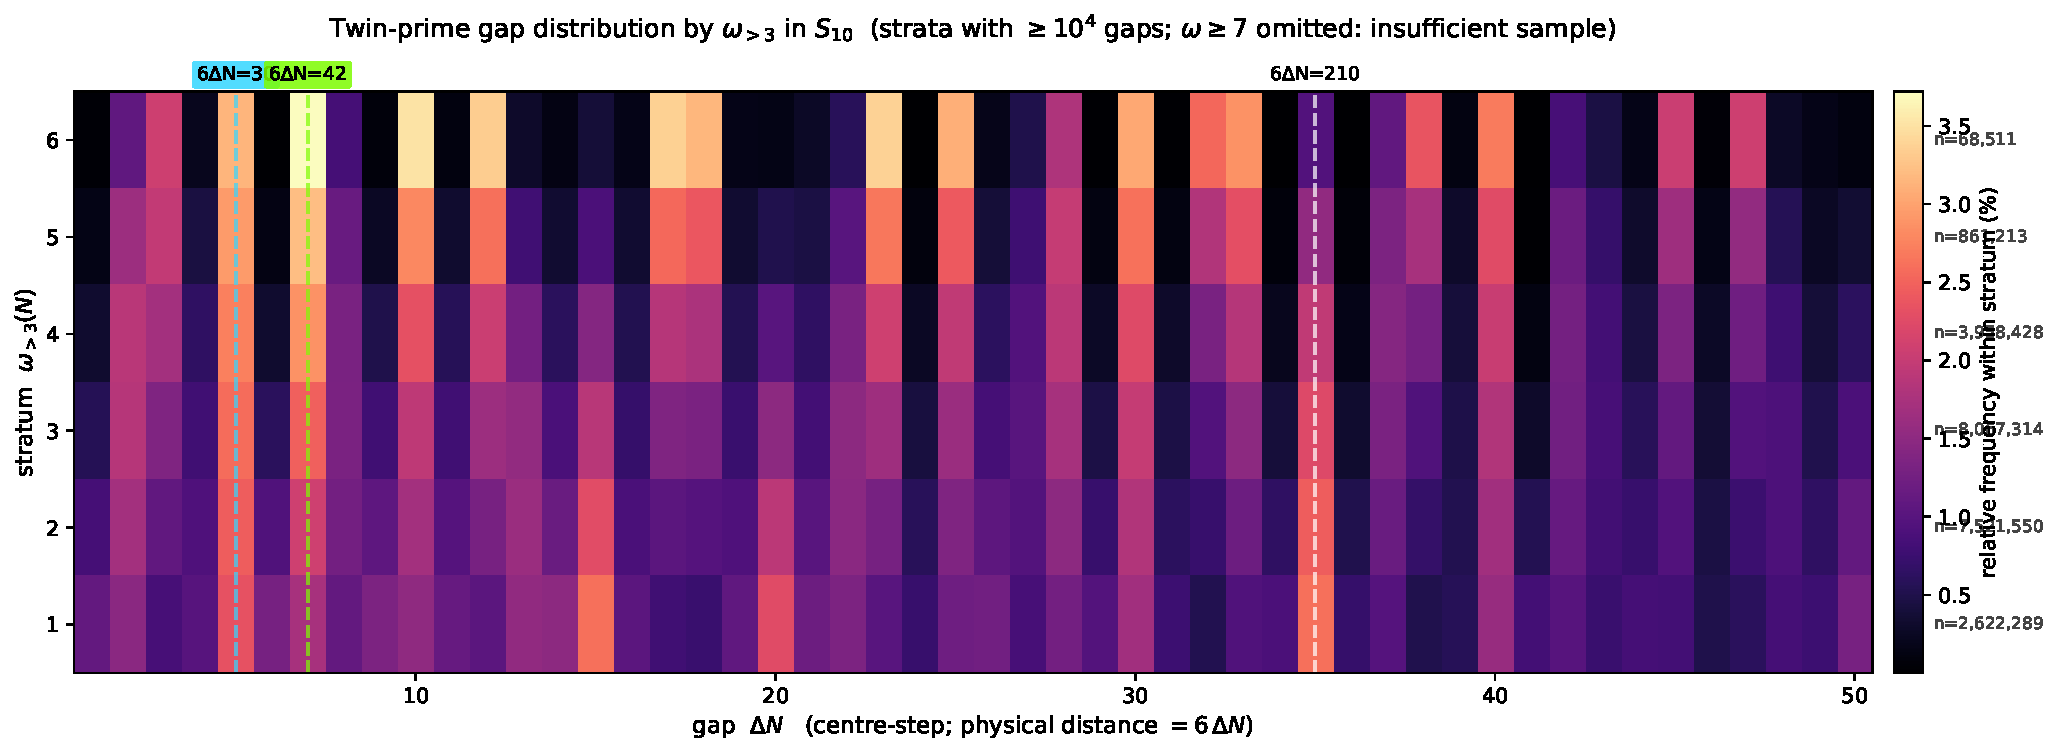
\includegraphics[width=\textwidth]{fig_paper2_gap_by_omega.pdf}
\caption{Twin-gap distribution by stratum $\omega_{>3}$ in $S_{10}$
(row-normalised; strata with $\ge10^4$ gaps). The $6\Delta N=210$ column
(rightmost guide) is bright at low $\omega$ and fades upward, while the
$6\Delta N=42$ column brightens upward. Sample sizes per stratum are annotated.}
\label{fig:heat}
\end{figure}

The two principal gaps move in opposite directions, monotonically
(Table~\ref{tab:resid}): the preference for $6\Delta N=42$ rises with $\omega$
and that for $210$ falls. The effect is not subtle---each spans roughly a factor
of two---and it is stable across three independent shells differing by
$\sim\!64\times$ in sample size.

\begin{table}[h]\centering
\begin{tabular}{llcccccc}
\toprule
$6\Delta N$ & shell & $\omega{=}1$ & 2 & 3 & 4 & 5 & 6\\
\midrule
\multirow{3}{*}{$42$}
 & $S_8$  & 0.72 & 0.90 & 1.12 & 1.31 & 1.54 & --\\
 & $S_9$  & 0.73 & 0.90 & 1.06 & 1.30 & 1.42 & 1.38\\
 & $S_{10}$ & 0.73 & 0.88 & 1.05 & 1.22 & 1.37 & 1.55\\
\midrule
\multirow{3}{*}{$210$}
 & $S_8$  & 1.14 & 1.06 & 0.94 & 0.83 & 0.53 & --\\
 & $S_9$  & 1.14 & 1.07 & 0.98 & 0.82 & 0.61 & 0.21\\
 & $S_{10}$ & 1.15 & 1.07 & 0.99 & 0.87 & 0.68 & 0.41\\
\bottomrule
\end{tabular}
\caption{Stratified residual $r(g\mid\omega)$ at the two principal gaps, across
three shells. Monotone, opposing, and scale-stable.}
\label{tab:resid}
\end{table}

\subsection{Controls}
The effect is not an artefact of the three obvious confounders, each checked
explicitly:
\begin{enumerate}[label=(\arabic*)]
  \item \textbf{Not noise:} reproduces across $S_8,S_9,S_{10}$
        (Table~\ref{tab:resid}) with near-identical values.
  \item \textbf{Not a size effect:} re-normalising each stratum by its own
        fitted geometric envelope (absorbing that stratum's mean gap) does not
        flatten the trend; the residual span is unchanged or slightly larger.
  \item \textbf{Not merely the Part~I scalar density:} the fitted gap-decay rate
        $a_\omega$ \emph{decreases} with $\omega$ while the twin density rate
        \emph{increases}, so $a_\omega$ is not a function of density alone
        ($a_\omega/\rho_\omega:0.32\to0.11$).
\end{enumerate}
Crucially, the unconditional Hardy--Littlewood series cannot produce \emph{any}
of this: $\mathfrak{S}(\Delta N)$ depends only on $\Delta N$. The shift must come
from a conditional mechanism, to which we now turn.

\input{paper2_section3_body}

\section{Conclusion}

Part~I established that the factorisation of the centre controls \emph{how many}
twin primes occur, through the scalar enrichment $E(N)$. This paper shows it also
controls \emph{how they are spaced}: the twin-gap distribution carries a
monotone, scale-stable dependence on $\omega_{>3}(N)$ that the unconditional
Hardy--Littlewood/jumping-champion framework---gap-only by construction---cannot
generate. We traced the effect to a first-order congruence-lockdown mechanism,
in which each prime factor of the centre forbids two gap residues, and verified
against $S_9$ data that it reproduces the rise of the short primorial gaps $42$
and $30$ and the collapse of the absolute survival of $210$. A real residual at
high arithmetic pressure remains beyond the first-order mechanism; together with
the closed-form conditional gap singular series $\mathfrak{S}_\omega(\Delta N)$,
it is left as a well-posed problem. The arc from Part~I to Part~II is thus from a
local density law to its imprint on the spacing structure---a conditional,
factor-resolved refinement of the classical gap statistics, demonstrated on
$\sim\!2.4\times10^{7}$ twin centres and offered, with its open residual, to
analytic number theory.

\paragraph{Data and code availability.}
All twin-centre data, verification scripts (gap statistics, Hardy--Littlewood
comparison, size and density controls, and the congruence-lockdown model), and
the figure-generating code are openly available~\cite{repo2}; the full scan is
reproducible from a single segmented-sieve program with deterministic primality,
self-verified against an independent factoriser.

\begin{thebibliography}{9}
\bibitem{ChenI} R.~Chen, \emph{Prime distribution on the $6N$ skeleton: a
factor-resolved local model for the conditional density of twin primes}, (Part~I),
Zenodo, doi:10.5281/zenodo.20470367 (2026).
\bibitem{ORW} A.~Odlyzko, M.~Rubinstein, M.~Wolf, \emph{Jumping champions},
Experiment.\ Math.\ \textbf{8} (1999), 107--118.
\bibitem{GL} D.~A.~Goldston, A.~H.~Ledoan, \emph{Jumping champions and gaps
between consecutive primes}, Int.\ J.\ Number Theory \textbf{7}(6) (2011),
1413--1421; doi:10.1142/S179304211100471X; arXiv:0910.2960.
% volume 7(6) 2011 and start page 1413 verified (World Scientific / NSF); end page 1421 self-consistent (9-pp article) but confirm on publisher page.
\bibitem{KP1} P.~F.~Kelly, T.~Pilling, \emph{Characterization of the
distribution of twin primes}, arXiv:math/0103191 (2001).
\bibitem{KP2} P.~F.~Kelly, T.~Pilling, \emph{Implications of a new
characterisation of the distribution of twin primes}, arXiv:math/0104205 (2001).
\bibitem{GGPY} D.~A.~Goldston, S.~W.~Graham, J.~Pintz, C.~Y.~Yıldırım,
\emph{Small gaps between primes or almost primes}, Trans.\ Amer.\ Math.\ Soc.\
\textbf{361}(10) (2009), 5285--5330; MR2515812; doi:10.1090/S0002-9947-09-04788-6;
arXiv:math/0506067.
\bibitem{Sono} K.~Sono, \emph{Small gaps between the set of products of at most
two primes}, J.\ Math.\ Soc.\ Japan \textbf{72}(1) (2020), 81--118;
doi:10.2969/jmsj/74937493; arXiv:1605.02920.
\bibitem{Dolgikh} S.~Dolgikh, \emph{Prime harmonics and twin prime
distribution}, Cambridge Open Engage, working paper, version~2 (2020),
doi:10.33774/coe-2020-c9x75-v2.
% TODO(author): confirm DOI and version on the Cambridge Open Engage page (not independently verified here).
\bibitem{Pusz} W.~Puszkarz, \emph{Statistical bias in the distribution of prime
pairs and isolated primes}, arXiv:1807.00406 (2018).
\bibitem{HL} G.~H.~Hardy, J.~E.~Littlewood, \emph{Partitio Numerorum III}, Acta
Math.\ \textbf{44} (1923), 1--70.
\bibitem{repo2} R.~Chen, \emph{$6N$ twin-prime gap data and code} (Part~II),
\url{https://github.com/Ruqing1963/6N-twin-prime-gap-omega-dependence} (2026).
\end{thebibliography}

\end{document}
